\documentclass{article}

\usepackage[english]{babel}
\usepackage[margin=3cm]{geometry}
\usepackage{graphicx}
\usepackage{float}
\usepackage{caption}
\usepackage{hyperref}
\usepackage{amsmath}
\usepackage{wrapfig}
\usepackage[parfill]{parskip}

% fonts
\usepackage[T1]{fontenc}
\usepackage{helvet}
\renewcommand{\familydefault}{\sfdefault}

\graphicspath{{img/}}

% theorem environment
\usepackage{amssymb}

\newtheorem{theorem}{Definitie}[section]

\usepackage{enumitem}

\newenvironment{thmenum}
 {\begin{enumerate}[label=\upshape\bfseries(\roman*)]}
 {\end{enumerate}}


% code
\usepackage{minted}
\setminted{frame=single,framesep=3pt,linenos}
\usepackage{upquote}
\usepackage{color}

\begin{document}

\begin{titlepage}
    \author{Tuur Vanhoutte}
    \title{Linux OS}
\end{titlepage}

\pagenumbering{gobble}
\maketitle
\newpage
\tableofcontents
\newpage

\pagenumbering{arabic}

\section{Introductie}

\subsection{Verschil Server \& Workstation}

\subsubsection{Server}

\begin{itemize}
    \item Deliver services to (multiple) users
    \item Focussed: only this and nothing else
    \item Secure
    \item No GUI, everything happens through the commandline
    \item $\Rightarrow$ as small a footprint as possible
\end{itemize}

\subsubsection{Workstation}

\begin{itemize}
    \item Use services
    \item Create documents
    \item Look for information
    \item Consume multimedia
    \item GUI
    \item $\Rightarrow$ Large footprint
\end{itemize}

\subsection{Extra information/resources}

\begin{itemize}
    \item The Linux Documentation Project: \url{http://tldp.org}
    \item Pluralsight LPIC-1: Linux Professional Institute Certification: \url{https://www.pluralsight.com/paths/lpic-1}
    \item The Arch Linux Wiki is one of the most extensive sources of info about Linux: \url{https://wiki.archlinux.org}
    \begin{itemize}
        \item In this module we will use Debian, not Arch, but many things are very similar
    \end{itemize}
    \item Google
\end{itemize}

\subsection{What is Linux?}

\subsubsection{What is an operating system (OS)?}

\begin{theorem}[Operating System]
An operating system, or OS, is software that communicates with the hardware
and alows other programs to run. 

It is comprised of system software = the fundamental files your computer needs to function.
\end{theorem}


\textcolor{red}{Linux is NOT an operating system: Linux = the \underline{\textbf{kernel}}}

\subsubsection{What is a Kernel?}

\begin{theorem}[Kernel]
The kernel is software that is the core of a computer's operating system, with complete control over the system.

It is the first program loaded on start-up. 

It handles\dots: 

\begin{itemize}
    \item \dots the rest of the startup
    \item \dots input/output requests from software, translating them into instructions for the CPU
    \item \dots memory
    \item \dots peripherals
\end{itemize}
\end{theorem}


\subsection{GNU Operating System}

\begin{theorem}[GNU]
GNU = GNU's Not Unix (recursive algorithm)

Founded by Richard Stallman (ex-MIT, founder of the Free Software Foundation), 1984

Goal: completely free Operating System
\end{theorem}

\subsection{Linux, the kernel}

By Linus Torvalds (Finland), 1991

\begin{itemize}
    \item Own personal development, not initially intended to distribute
    \item Interest from other developers, mainly to use with GNU OS
    \item Meanwhile contributions of over 12000+ developers
    \item 492 of top-500 supercomputers in the world run Linux
    \item Basis for Android, Chrome OS
\end{itemize}

Linux = the kernel

GNU = OS-tools around the kernel

$\Rightarrow$ \textbf{GNU/Linux}

\subsubsection{Distributions}

\begin{theorem}[Distribution]
A Linux distribution (or distro for short) is GNU/Linux + extra tools and applications to create a full-fledged OS.

That distribution can be easily copied and installed to other computers.
\end{theorem}

\begin{itemize}
    \item RedHat (CentOS)
    \item Debian (Ubuntu)
    \item Arch Linux
    \item Void Linux
    \item Gentoo
    \item Pop! OS
\end{itemize}

\begin{figure}[H]
    \centering
    \includegraphics[width=0.75\textwidth]{redhat-vs-debian-tree.png}
    \caption{\url{https://upload.wikimedia.org/wikipedia/commons/1/1b/Linux_Distribution_Timeline.svg}}
\end{figure}

\url{https://en.wikipedia.org/wiki/List_of_Linux_distributions}

\subsection{Open Source}

\begin{theorem}[Open Source]
Open source software is software of which the code is licensed to be open to everyone. 

Anyone can use, change, distribute the software. This allows code to be developed in a public manner.
\end{theorem}

\textbf{\textcolor{red}{OPEN SOURCE DOES NOT MEAN FREE}}

\subsubsection{Commercial distributions}

= Open source, non-free distributions

\begin{itemize}
    \item SUSE Linux Enterprise Server (SLES)
    \item SUSE Linux Enterprise Desktop (SLED)
    \item Red Hat Enterprise Linux (RHEL)
    \item Oracle Enterprise Linux
\end{itemize}

Commercial distributions have official support channels.

$\Rightarrow$ You're not paying for the operating system, you're paying for the support.

\subsubsection{In this course: Debian}


\begin{itemize}
    \item Current version: 10.7
    \item Forms the basis of many others: Ubuntu, Raspbian, Knoppix, Linux Mint
    \item Available on many platforms: Intel x86, AMD64, Intel64, ARM, MIPS, Power Systems, \dots
\end{itemize}

\section{Debian Installation}

\textbf{See Labs for detailed Installation tutorial}

\subsection{Networking in Linux (with VMWare)}

\begin{itemize}
    \item VMWare presents ethernet adapter
    \item During creation of virtual machine: MAC-address is created
    \item During installation: network configuration through DHCP
    \begin{itemize}
        \item IPv4-address
        \item Default gateway
        \item DNS-server
        \item \underline{Optional:} proxy-server
    \end{itemize}
\end{itemize}

\subsection{Users in Linux}

\begin{itemize}
    \item Linux is multi-user from the ground up
    \begin{itemize}
        \item Multiple users can be active at the same time
    \end{itemize}
    \item `Administrator'-user is called root
    \item Each user has a user-ID (uid)
    \begin{itemize}
        \item root has uid=0
        \item uid=0 has all rights
    \end{itemize}
    \item Each user has a home-directory
\end{itemize}

\subsection{Disks, partition, filesystems}

\begin{itemize}
    \item Our VM has 1 disk
    \begin{itemize}
        \item Presented on the SCSI-bus
        \item First disk on SCSI-bus: \textbf{sda}
        \item Then sdb, sdc, \dots
    \end{itemize}
    \item Disk = concatenation of blocks
    \item Divide blocks in collections (=partitions)
    \begin{itemize}
        \item 1st partition: sda1
        \item 2nd partition: sda2
        \item \dots
    \end{itemize}
    \item 2 types of partitions
    \begin{itemize}
        \item Primary
        \item Extended
    \end{itemize}
\end{itemize}

\subsubsection{Partitions}

Primary partition

\begin{itemize}
    \item A filesystem can be created inside this
    \item Up to 4 primary partitions
\end{itemize}

Extended Partition

\begin{itemize}
    \item `Logical' partitions can be created inside this
\end{itemize}

Our setup:

\begin{itemize}
    \item sda1: primary partition
    \item sda2: extended partition
    \item sda5: `logical' partition inside extended partition sda2
\end{itemize}

\begin{figure}[H]
    \centering
    \includegraphics[width=0.3\textwidth]{partitions.png}
    \caption{Our setup}
\end{figure}

\subsection{MBR <> GPT}

\subsubsection{MBR}

We use the MBR Partitioning scheme

\begin{theorem}[MBR]
MBR, or Master Boot Record, is a special type of boot sector at the start of a disk.

It contains: 

\begin{itemize}
    \item a set of instructions necessary to boot operating systems.
    \item info about how partitions are placed on disk
\end{itemize}


\end{theorem}

Limitations:

\begin{itemize}
    \item Maximum disks of 2TB
    \item 32-bit for number of logical sectors
    \item Common sector size: 512 bytes
    \item $2^{32} \cdot 512\ \text{bytes} = 4294967296 \cdot 512\ \text{bytes} \approx 2\text{TB}$
    \item Maximum amount of primary partitions = 4
\end{itemize}

BIOS can boot from a disk with MBR partitioning

\subsubsection{GPT}

\begin{theorem}[GPT]
GPT, or GUID Partition Table, is a standard for the layout of partition tables on a disk.
It's an alternative to MBR.

It uses unique identifiers (GUIDs) 
\end{theorem}

\begin{itemize}
    \item BIOS cannot boot from a disk with GPT-partitioning: UEFI required when using GPT
    \item GPT allows disks larger than 2TB
\end{itemize}

\begin{theorem}[UEFI]
UEFI, or Unified Extensible Firmware Interface, is a newer firmware interface by Intel (90's) that replaces the BIOS interface by IBM (70's).
\end{theorem}

\textbf{How does it work?}

\begin{itemize}
    \item Disk = collection of blocks
    \item Group of blocks together = sector
    \item Common sector size: 512 bytes
    \item Sectors indicated with Logical Block Addresses (LBA)
    \item MBR in LBA 0
    \item GPT headers in LBA 1
    \item Partition tabel right after that
\end{itemize}




\subsubsection{Bootstrap procedure}

\begin{enumerate}
    \item Motherboard gets electricity
    \item Mini-loader hardcoded in memory
    \begin{itemize}
        \item BIOS gets loaded
    \end{itemize}
    \item Boot media are consulted
    \item First boot medium, first sectors are being read $\Rightarrow$
    \item MBR contains a bit-more-advanced loader: GRUB
    \begin{itemize}
        \item \underline{GR}and \underline{U}nified \underline{B}ootloader
    \end{itemize}
    \item This loader loads a more advanced loader (GRUB second stage bootloader)
    \item The OS is loaded
\end{enumerate}

\subsubsection{Linux boot process}

6 high level steps

\begin{itemize}
    \item BIOS (Basic Input/Output System) - loads MBR
    \item MBR (Master Boot Record) - loads GRUB
    \item GRUB (Grand Unified Bootloader) - loads kernel
    \item Kernel - executes /sbin/init
    \item Init - executes runlevel programs
    \item Runlevel - programs from /etc/rc.d/rcXX.d are started
\end{itemize}

\subsubsection{BIOS <> UEFI}

\begin{itemize}
    \item Recent systems use UEFI, not BIOS
    \item UEFI is required to boot from GPT-disk
    \item Linux has no trouble working with UEFI
\end{itemize}

\textbf{So why will we use MBR?}

\begin{itemize}
    \item Virtualisation is the norm
    \item Virtual machines typically have small disks
    \item Small disks are MBR partitioned
\end{itemize}



\subsection{Filesystems}

\subsubsection{Windows}

\begin{itemize}
    \item FAT (1977)
    \item FAT32 (1996)
    \item NTFS (1993)
    \item ReFS (2012)
\end{itemize}

\subsubsection{Linux}

\begin{itemize}
    \item Ext (1992)
    \item Ext2 (1993)
    \item Ext3 (2001)
    \item Ext4 (2008)
    \item ZFS (2005)
    \item BtrFS (2007)
\end{itemize}

\subsubsection{Swap}

= Paging

\begin{itemize}
    \item Free up physical memory (RAM) by moving pages to slower storage (storage disks instead of RAM)
    \item Page out $=$ memory page moves to swap
    \item "Swapiness"
    \begin{itemize}
        \item = parameter between 0 and 100
        \item = how quickly linux will swap
        \begin{itemize}
            \item 0 = very conservative
            \item 100 = very agressive
        \end{itemize}
    \end{itemize}
    \item Windows uses a swap file (pagefile.sys)
    \item Linux uses a swap partition
\end{itemize}

\subsection{File structure}



\begin{figure}[H]
    \centering
    \includegraphics[width=0.4\textwidth]{linux-filestructure.png}
    \caption{Linux uses a tree structure}
\end{figure}

\begin{figure}[H]
    \centering
    \includegraphics[width=0.5\textwidth]{windows-filestructure.png}
    \caption{Windows uses a similar structure, but every volume uses a letter.}
\end{figure}

\begin{figure}[H]
    \centering
    \includegraphics[width=0.5\textwidth]{linux-filestructure2.png}
    \caption{With linux, volumes are `mounted' to folders somewhere under root /}
\end{figure}

\subsection{Configuration}

\subsubsection{Packages}

\begin{itemize}
    \item Tools and applications are build up by files
    \item All files belonging to 1 application are bundled in a package
    \item Packages in debian have the .deb extension
\end{itemize}

Repositories

\begin{itemize}
    \item Packages are collected in repositories
    \item Are made available through the internet
    \item Packages have dependencies
\end{itemize}

\subsubsection{Package management}

Debian: dpkg \& apt (Advanced Package Tool)

\begin{itemize}
    \item dpkg: Install, remove, give info about .deb packages
    \begin{itemize}
        \item dpkg -l = lists packages 
    \end{itemize}
    \item apt: Get packages from a repository and install, remove, give info, ...
    \begin{itemize}
        \item apt update
        \begin{itemize}
            \item Contact the repositories
            \item Get most recent list of packages and versions
        \end{itemize}
        \item apt upgrade
        \begin{itemize}
            \item Of the packages which are more recent in the repositories compared to what is installed: install newest version
        \end{itemize}
        \item apt install <xyz>
        \begin{itemize}
            \item Download package <xyz> from the repository
            \item Check the dependencies and download depending packages
            \item Install package <xyz> and all corresponding dependencies
        \end{itemize}
    \end{itemize}
\end{itemize}

Which repositories? See /etc/apt/sources.list for the list of repositories. You can add/remove/change repositories in this file.

\subsubsection{Useful packages}

\begin{itemize}
    \item open-vm-tools
    \item vim
    \item sudo
    \item tcpdump
\end{itemize}

Install multiple pacakges in one command: apt install vim sudo tcpdump ntp

\subsection{Shutdown of VM}

\begin{itemize}
    \item Power button (=ACPI shutdown)
    \item Shut down operating system only
    \begin{itemize}
        \item = halt
    \end{itemize}
    \item Shut down operating system and VM, multiple ways:
    \begin{itemize}
        \item shutdown -P now
        \item init 0
        \item poweroff
    \end{itemize}
    \item Reboot
    \begin{itemize}
        \item reboot
        \item init 6
        \item shutdown -r now
    \end{itemize}
\end{itemize}

\subsection{Basic network}

\begin{itemize}
    \item No GUI $\Rightarrow$
    \item Layer 1: Physical (VMWare virtual network)
    \item Layer 2: Datalink (Ethernet \& MAC address)
    \item Layer 3: Network (IPv4)
    \item Layer 4: Transport (Transport Control Protocol (TCP), User Datagram Protocol (UDP))
    \item Layer 5: Application (SSH, HTTP, \dots)
\end{itemize}

\subsubsection{Basic networking commands}

\begin{itemize}
    \item arp
    \item ping
    \item route
    \item bmon
\end{itemize}

\subsection{Services}

\begin{itemize}
    \item Processes that `listen' on the network
    \begin{itemize}
        \item TCP or UDP port
    \end{itemize}
    \item Overview of currently running / listening services: ss command
    \begin{itemize}
        \item ss -tulpn
        \item t: show TCP
        \item u: show UDP
        \item l: show listening
        \item p: show process ID
        \item n: no name-resolving
    \end{itemize} 
\end{itemize}

\subsection{Wooclap Questions}

\begin{itemize}
    \item Why do we talk about GNU/Linux?
    \item What is a kernel?
    \item What is the difference between Open Source and free?
    \item How is the Administrator user called? What is its uid?
    \item What is MBR?
    \item What are the limitations of MBR? (Solution?)
    \item What is swap? What is swappiness?
    \item What is a package?
    \item What is a repository?
    \item What is a dependency?
    \item What is a package manager?
    \item What is the difference between 'apt update' and 'apt upgrade'
    \item Which protocol makes the link between MAC address \& IP address?
    \item Which command gives you the current ARP-table?
    \item What are the 5 layers of the TCP/IP network model?
    \item How do you find the MAC-address of a network interface?
    \item Put Linux boot process in correct order (6 levels)
    \item What is a linux distribution?
\end{itemize}

\section{File structure}

\begin{itemize}
    \item Tree structure
    \begin{itemize}
        \item Leaves = files
        \item Branches = directories
        \item The tree is inverted, root = /
    \end{itemize}
    \item Everything is a file (even devices, random numbers, and RAM) under 1 root
    \item This is in contrast to Windows, where every volume is a root.
\end{itemize}

\begin{figure}[H]
    \centering
    \includegraphics[width=0.4\textwidth]{linux-filestructure.png}
    \caption{}
\end{figure}



\subsection{Intermezzo: single user mode}

\begin{itemize}
    \item Linux (the kernel) is built up as a multi-user system from the beginning
    \item Standard behaviour = multi-user
    \item But: also possible to boot in single-user mode
    \begin{itemize}
        \item No daemons, no multiple logins
        \item Sometimes called \textbf{Maintenance mode}
    \end{itemize}
    \item Examples of usage
    \begin{itemize}
        \item Filesystem repairs
        \item Upgrade of distribution
        \item Password recovery
        \item Adjustments to the root filesystem
        \item Forensics after security incident
    \end{itemize}
\end{itemize}

\subsubsection{Runlevels}

= predefined operating system status

\begin{itemize}
    \item Is presented with a number
    \item Linux has 7 runlevels:
    \begin{itemize}
        \item 0 = system halt (= VM shutdown)
        \item 1 = single user
        \item 2 = multi-user, no NFS (no network services, not often used)
        \item 3 = multi-user, CLI (Command Line Interface)
        \item 4 = self-definable
        \item 5 = multi-user, GUI (Graphical User Interface, if installed)
        \item 6 = reboot
    \end{itemize}
\end{itemize}

\subsection{Intermezzo: Add disk}

\textbf{Add a new disk without shutting down the system}

\begin{enumerate}
    \item Adjust VM: add disk
    \item Detect added disk
    \item Partition disk
    \begin{itemize}
        \item fdisk (for MBR)
        \item parted (for GPT)
    \end{itemize}
    \item Create filesystem
    \begin{itemize}
        \item Partition = collection of blocks (sectors)
        \item Not usable for the OS $\Rightarrow$ create filesystem
        \item mkfs.ext4 /dev/sdb1
        \begin{figure}[H]
            \centering
            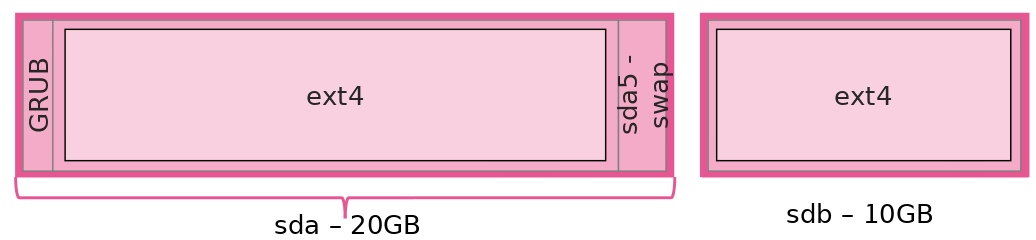
\includegraphics[width=0.7\textwidth]{create-filesystem.png}
            \caption{}
        \end{figure}
    \end{itemize}
    \item Mount filesystem
    \begin{itemize}
        \item mkdir /mnt/datadisk
        \item mount /dev/sdb1 /mnt/datadisk
        \item see if it worked: df -h
    \end{itemize}
\end{enumerate}

\textbf{For detailed steps: see labs!}


\subsubsection{What after a reboot?}

Use /etc/fstab = a file that contains what needs to be mounted at boot

\begin{itemize}
    \item Device (/dev/sdXY or UUID) 
    \item Mountpoint (/mnt/folder)
    \item Type of filesystem (ext4, ntfs, \dots)
    \item Options
\end{itemize}


\subsection{Navigate through the tree}

\begin{itemize}
    \item pwd
    \begin{itemize}
        \item Print working directory
        \item Shows where in the tree you are
    \end{itemize}
    \item ls
    \begin{itemize}
        \item Show a list of files in the working directory
        \item ls -la : 10 characters at the beginning of each line. The d == directory (see later)
    \end{itemize}
    \item When you login, you are in your home directory
    \item / (= the filesystem root) is not the same as /root (the home directory of the root user)
    \item . = current directory
    \item .. = the directory one higher
\end{itemize}

\subsubsection{Relative vs absolute path}

Relative paths:

\begin{itemize}
    \item cd .. = go to the directory above the current directory
    \item cat ../etc/issue = go to the etc directory, one directory above the current directory. Open the issue file
\end{itemize}

Absolute paths:

\begin{itemize}
    \item cd / = go to the root directory
    \item cat /etc/issue = go to the etc/ directory under / (root)
\end{itemize}

\subsection{Filesystem Hierarchy Standard (FHS)}

\begin{itemize}
    \item Describes how the filesystem in Linux is build up
    \item Maintained by the Linux Foundation
    \item Most recent version: v3.0 (2015)
\end{itemize}



\subsubsection{Rules in the standard}

\begin{itemize}
    \item / is the root of the tree structure
    \item /bin 
    \begin{itemize}
        \item essential binaries (executable files), required for single user mode
    \end{itemize}
    \item /boot
    \begin{itemize}
        \item the place on the filesystem where the boot files reside
        \item configuration files for GRUB
        \item kernels
        \item initrd
        \begin{itemize}
            \item initial RamDisk
            \item During boot a temporary root-filesystem is being created in RAM
            \item This is used so the kernel can load important modules, so it can then switch to the real root filesystem
            \item part of step 3 of the linux boot process (BIOS - MBR - GRUB - kernel - init - runlevel)
        \end{itemize}
    \end{itemize}
    \item /dev
    \begin{itemize}
        \item Devices get a place in the filesystem
        \begin{itemize}
            \item sda
            \item rtc
            \item random
            \item cpu
            \item urandom
            \item null
        \end{itemize}
        \item ls -lah /dev/
    \end{itemize}
    \item /etc
    \begin{itemize}
        \item Host-specific sytem-wide configuration files
        \item Configuration for this host, readable for the whole system
    \end{itemize}
    \item /home
    \begin{itemize}
        \item Each (non-system) user has a home directory
        \item except for root $\Rightarrow$ /root
    \end{itemize}
    \item /mnt
    \begin{itemize}
        \item (temporarily) `mounted' filesystems
        \begin{itemize}
            \item Network shares
            \item USB-disk
            \item DVD-ROM
            \item Extra disks
        \end{itemize}
        \item Some distributions use /media for this
    \end{itemize}
    \begin{figure}[H]
        \centering
        \includegraphics[width=0.3\textwidth]{linux-filestructure2.png}
        \caption{}
    \end{figure}
    
    \item /opt
    \begin{itemize}
        \item Optional application software packages
        \item Our installation $\Rightarrow$ no applications installed yet = empty (for now)
    \end{itemize}
    \item /proc
    \begin{itemize}
        \item Virtual filesystem
        \item Provides information about processes and the linux kernel
        \item cat /proc/cpuinfo
        \item cat /proc/sys/net/ipv4/ip\_forward
        \item cat /proc/partitions
    \end{itemize}
    \item /sbin
    \begin{itemize}
        \item Essential system binaries
        \item Only executable by root user
        \item fsck, init, route
    \end{itemize}
    \item /tmp
    \begin{itemize}
        \item Directory for temporary files
        \item Emptied at reboot (with most distributions)
    \end{itemize}
    \item /usr
    \begin{itemize}
        \item Read-only user data
        \item Constains most user (non-root) utilities and applications
    \end{itemize}
    \item /var
    \begin{itemize}
        \item Variable files
        \item Files that are expected to change continuously during normal system use
        \item Logs, spool files, temporary e-mail files, \dots
    \end{itemize}
\end{itemize}

\subsection{Some useful tips}

\subsubsection{History}

\begin{minted}{bash}
~# history

# shows a list of former commands executed by this user
# spans log-in sessions
# in reality, it shows the contents of the ~/.bash_history file
# if you use another shell like zsh, it's the ~/.zsh_history file
\end{minted}

CTRL + r:

\begin{itemize}
    \item Search the command history
    \item Show commands that match what you're typing
    \item repeatedly press ctrl+r to scroll through results
\end{itemize}


\subsubsection{Bind mount}

\textbf{Situation}

\begin{itemize}
    \item /mnt/storage is the normal mountpoint for other filesystems (e.g. SAN)
    \item Filesystem could not be mounted, but a process already started writing data
    \item $\Rightarrow$ this data arrives on the / filesystem under the directory /mnt/storage
    \item Problem fixed and filesystem can be mounted again $\Rightarrow$ mounted under /mnt/storage
    \item $\Rightarrow$ the already written data is now hidden
\end{itemize}

\textbf{The solution}

\begin{itemize}
    \item Create /mnt/storage and put some data in it
    \item Create a 1GB disk, ext4 formatted, mount under /mnt/storage $\Rightarrow$ data is now hidden
    \item Use mount -o bind to get data back without unmounting
\end{itemize}

\subsubsection{dd}

= Command to read or write bytes

\begin{minted}{bash}
# Example: overwrite first 2048 bytes of a disk with zeros
~# dd if=/dev/zero of=/dev/sdb count=4 bs=512
# Example: overwrite disk with random data when taking out of service
~# dd if=/dev/random of=/dev/sdb bs=1M
\end{minted}

\subsection{Wooclap Questions}

\begin{itemize}
    \item How do you ask the shell in which folder you are currently in?
    \item What is meant with the term 'runlevel' in Linux
    \item Describe single user mode with 1 word when you think of its primary use
    \item What is / are the most common runlevel(s) under linux? (So not all of them!)
    \item Where can you find the devices under Linux?
    \item What is the home directory of the root user?
    \item What command do we use to create a filesystem in a partition?
    \item What file do you need to edit to have a mounted filesystem available even after reboot?
    \item Where can you put temporary files in a linux system?
    \item How can you quickly search through your previously used commands?
    \item How do you quickly search through previously typed commands?
    \item What is swap?
    \item What are the limitations of MBR?
    \item What can you use a bind mount for?
\end{itemize}

\section{Filesystems}

\subsection{Introduction}

Books:

\begin{itemize}
    \item A group of letters together = a word
    \item A group of words together = a sentence
    \item A group of sentences together = a book
    \item A collection of books together = a library
    \item Books are ordered/sorted according to a certain system
    \begin{itemize}
        \item Best known: Dewey Decimal System
    \end{itemize}
\end{itemize}

Computers: 

\begin{itemize}
    \item Work with 0's and 1's
    \item 1 character in ASCII or ISO-8859-1 = 8bits (1 byte)
    \item 1 Unicode character in UTF-8: between 8 and 32 bits (4 bytes)
    \item Gets stored on block devices
    \begin{itemize}
        \item Hard devices, SSDs, RAMdisk, USB-stick
        \item The opposite of block devices = character devices 
    \end{itemize}
    \item System needs to organize this
\end{itemize}

\subsection{Blocks}

\begin{itemize}
    \item Disk = blocks
    \item Collection of blocks = sector (mostly 512 bytes)
    \item Collection of sectors = partition
    \item Partition not usable for an OS $\Rightarrow$ filesystem needed
\end{itemize}

\begin{theorem}[Filesystem]
    A filesystem is the methods and data structures that an operating system uses to keep track of files on a disk or partition; that is, the way the files are organized on the disk.
\end{theorem}

Several choices:

\begin{itemize}
    \item Ext2/3/4
    \item BrtFS
    \item ZFS
    \item \dots
\end{itemize}

\subsection{ext2/3/4}

Ext3 and Ext4 have journaling:

\subsubsection{Journaling}

\begin{itemize}
    \item Keeping track of changes that have not been committed to disk in a sort of 'diary'
    \item A kind of logbook of previous actions
    \item Why?
    \begin{itemize}
        \item Bring filesystem online faster after system crash or power failure
    \end{itemize}
\end{itemize}

\subsection{RAID}

\begin{theorem}[RAID]
    Redundant Array of Independant Disks (RAID) is a data storage virtualisation technology that combines multiple physical disk drive into one ore more logical units.

    Many purposes:

    \begin{itemize}
        \item Data redundancy
        \item Performance Improvement
        \item Both
    \end{itemize}
\end{theorem}

\subsubsection{RAID Controller}

\begin{itemize}
    \item Disks are connected to the controller
    \item The RAID controller displays the disks as 1 disk to the OS
    \item Nowadays, we call the RAID Controller the Host Bus Adapter (HBA)
    \item 
\end{itemize}

\subsubsection{RAID 0}

RAID level 0 uses striping:

\begin{theorem}[Striping]
    Data striping is the technique of segmenting logically sequential data (files) so that segments are stored on different physical storage devices

    Purpose:

    \begin{itemize}
        \item Increasing data throughput
        \item Balancing I/O load accross an array of disks
    \end{itemize}
\end{theorem}

\begin{figure}[H]
    \centering
    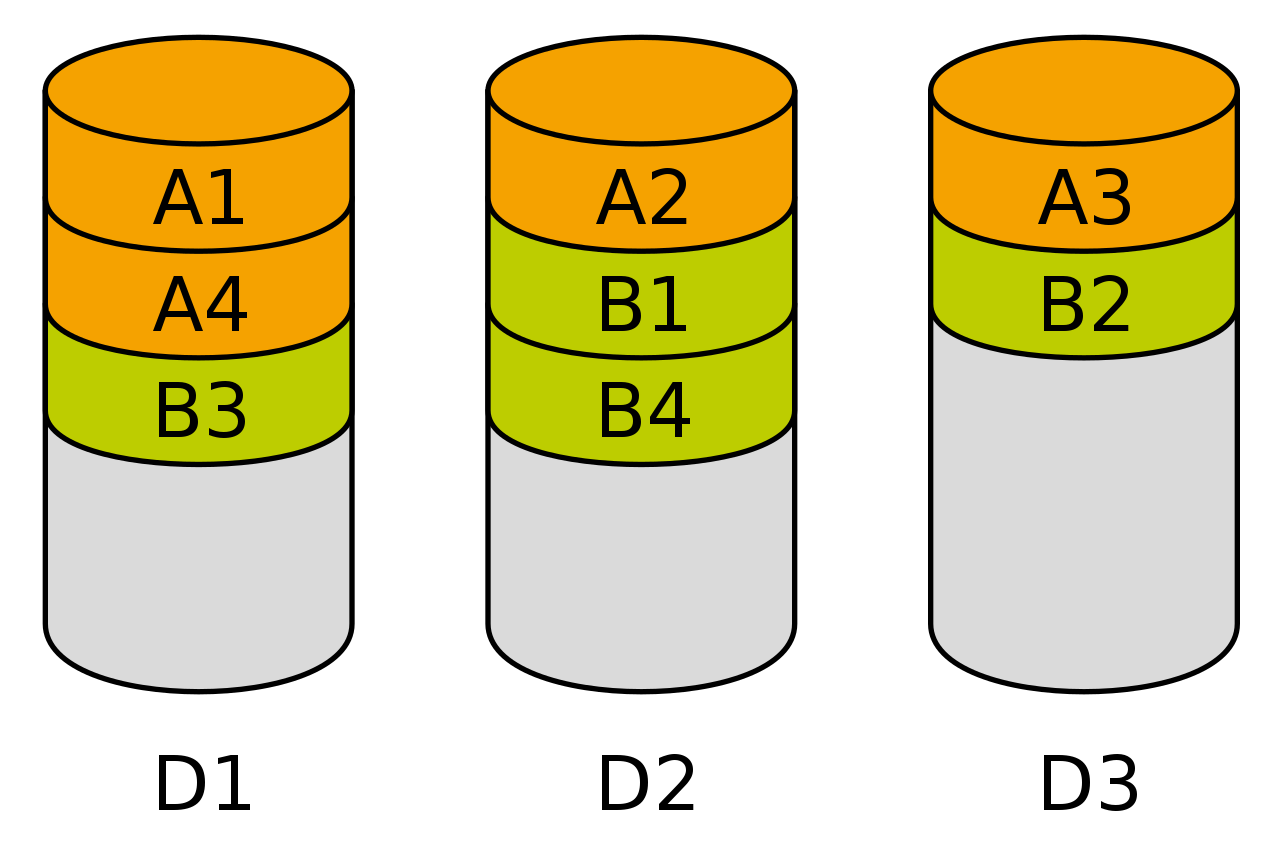
\includegraphics[width=0.3\textwidth]{raid-striping.png}
    \caption{Example: files A and B (4 blocks each) are spread over disks D1-D3}
\end{figure}


\subsubsection{RAID 1}

RAID level 1 uses mirroring:

\begin{theorem}[Mirroring]
    Disk mirroring is the replication of logical disk volumes onto seperate physical disks.

    Purpose:

    \begin{itemize}
        \item Continuous availability: in case of hardware failure, you always have a backup of your data
        \item Increasing read speeds
    \end{itemize}
\end{theorem}

\begin{figure}[H]
    \centering
    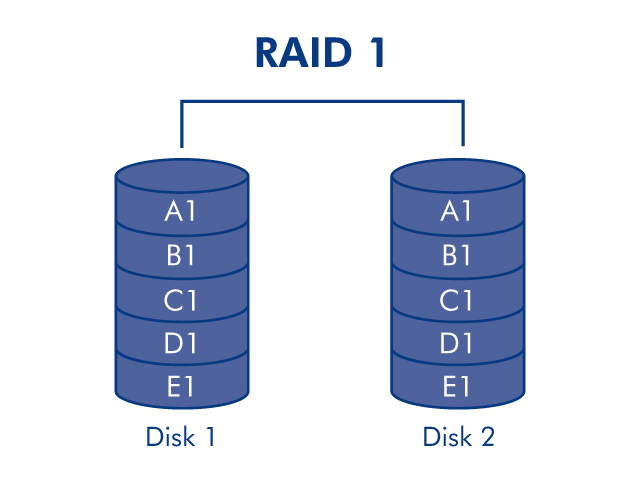
\includegraphics[width=0.3\textwidth]{raid-mirroring.png}
    \caption{RAID 1}
\end{figure}


\subsubsection{RAID 4}

\begin{itemize}
    \item If we have at least 3 disks
    \item For every block of data:
    \begin{itemize}
        \item Divide the block in 2 halves: A and B
        \item Write A to disk 1
        \item Write B to disk 2
        \item Write A+B to disk 3
    \end{itemize}
    \item $\Rightarrow$ RAID 4 is striping (disk 1 \& 2) with parity (disk 3)
    \item Capacity x2
    \item Read speed x2
    \item Write speed is limited, because of the need to write all parity data to a single disk
\end{itemize}

\begin{figure}[H]
    \centering
    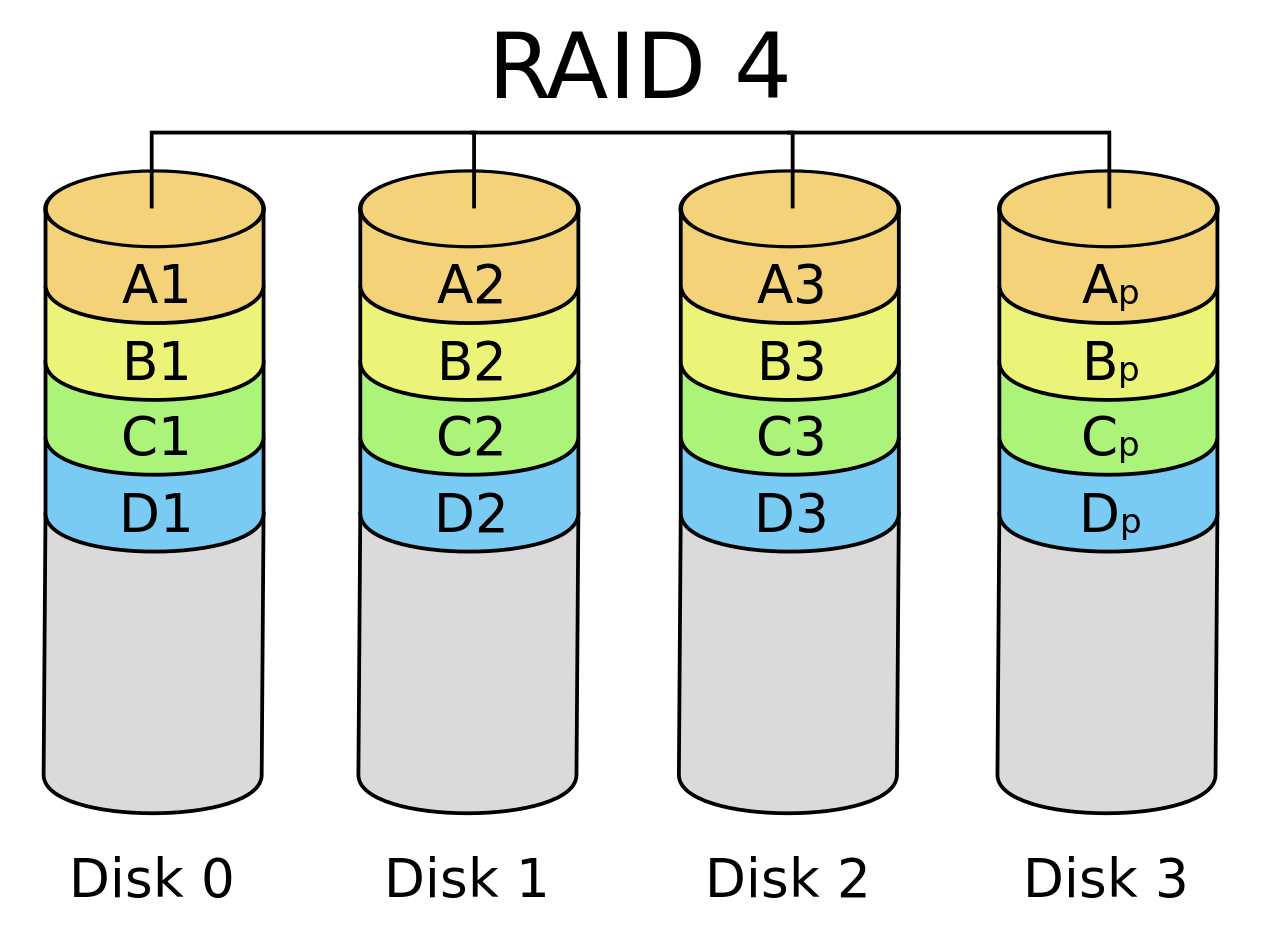
\includegraphics[width=0.3\textwidth]{raid-4.png}
    \caption{A RAID-4 setup with 4 disks. Disk 3 is the parity disk}
\end{figure}


\subsubsection{RAID 5}

RAID level 5 like RAID 4, but the parity is distributed.

\begin{itemize}
    \item This evens out the stress of a dedicated parity disk (RAID 4)
    \item Write performance is increased
\end{itemize}

\begin{figure}[H]
    \centering
    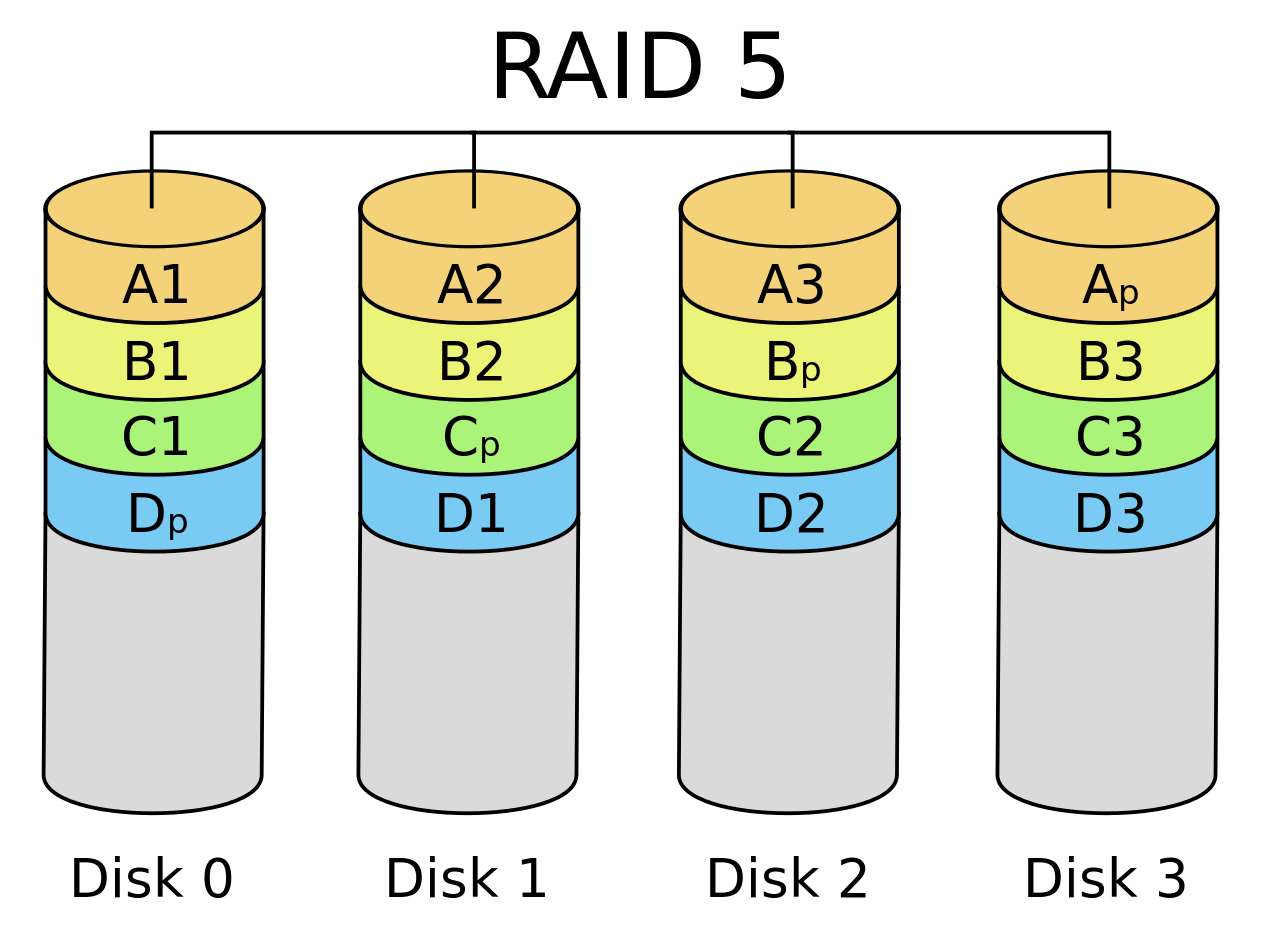
\includegraphics[width=0.3\textwidth]{raid-5.png}
    \caption{RAID-5: distributed parity with 4 disks}
\end{figure}


\subsubsection{RAID 6}

RAID level 6 like RAID 5, but with a second parity block.

\begin{figure}[H]
    \centering
    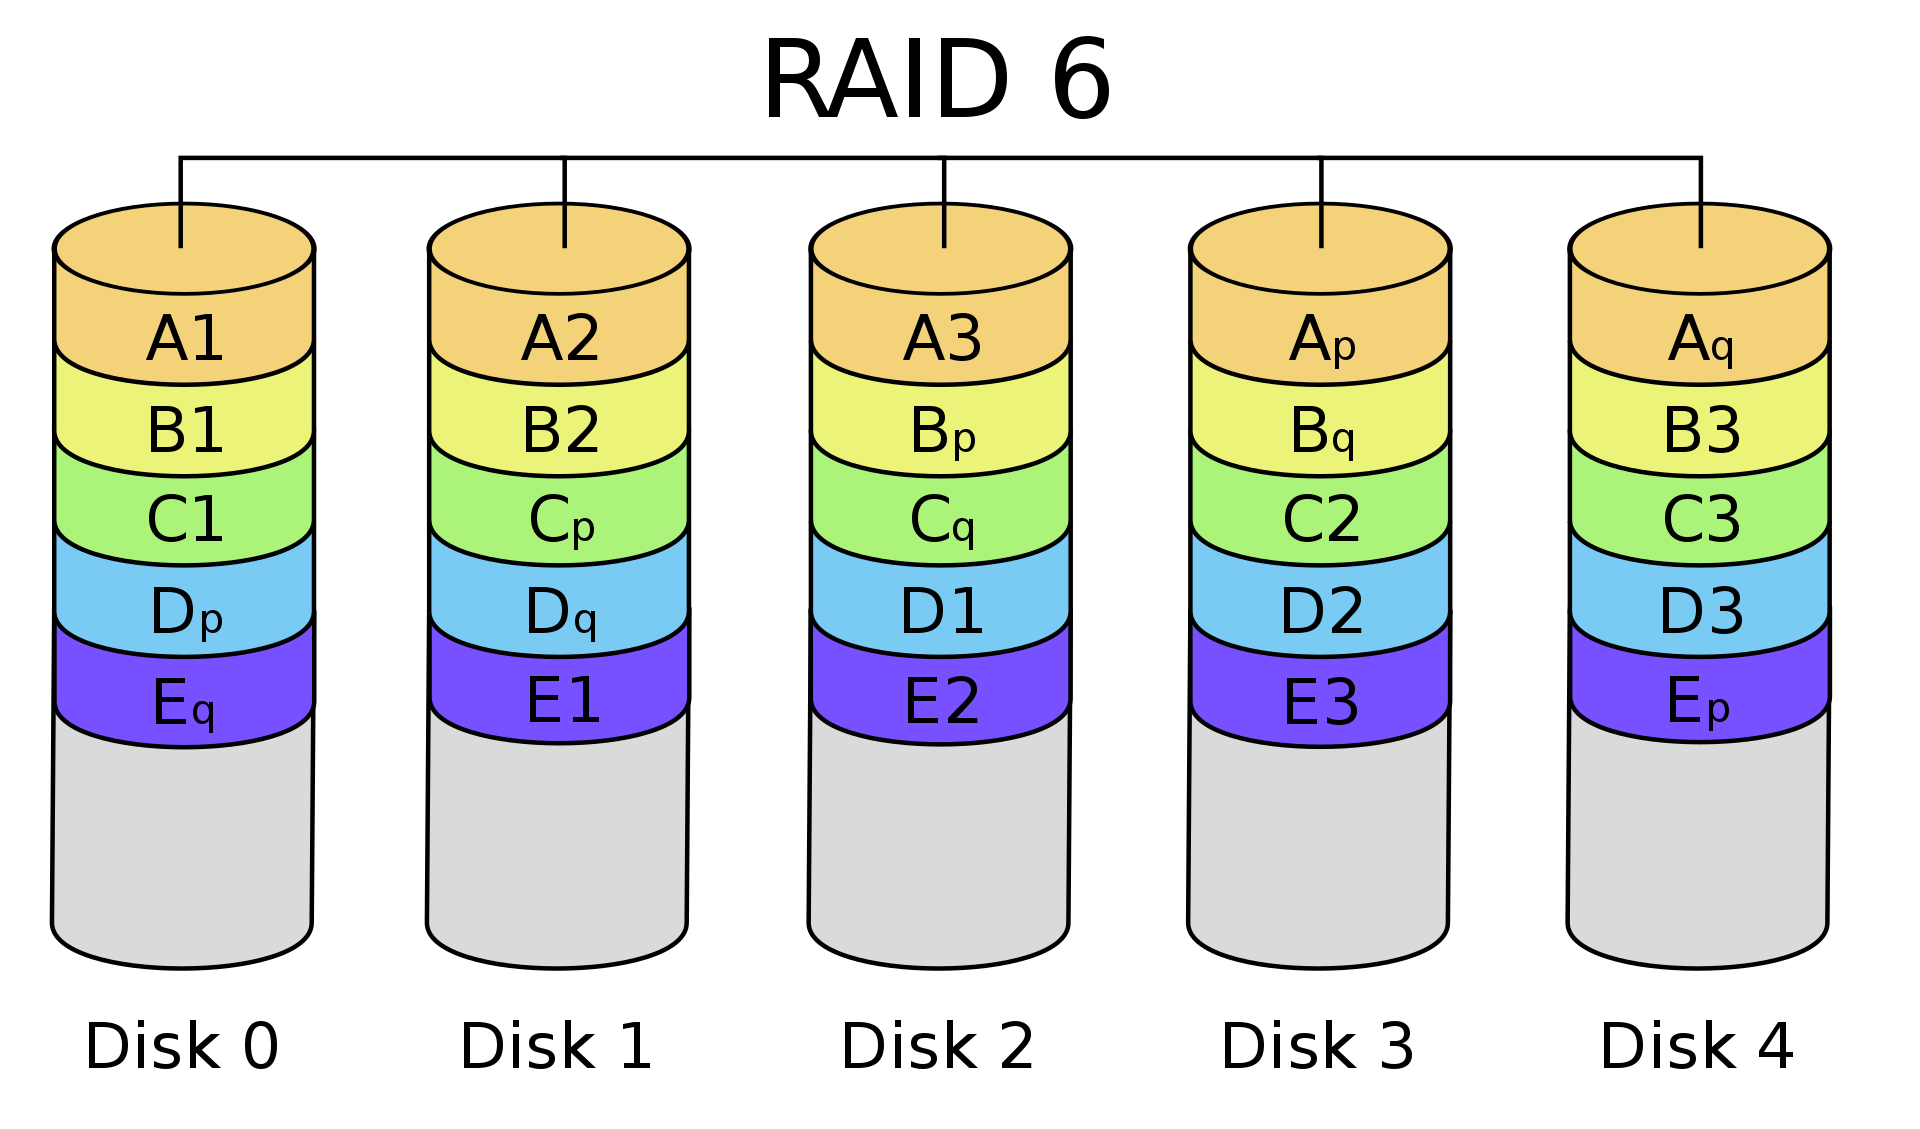
\includegraphics[width=0.3\textwidth]{raid-6.png}
    \caption{}
\end{figure}



\subsubsection{Disk failure}

For every RAID level, a certain amount of disks can fail without it becoming a problem:

\begin{itemize}
    \item RAID 0: no disks can fail: if any disk fails, you lose data
    \item RAID 1: Every disk except for one can fail
    \item RAID 5: 1 disk can fail
    \item RAID 6: 2 disks can fail
\end{itemize}

\subsubsection{Compound RAID levels}

Combining RAID levels is possible:

\begin{itemize}
    \item RAID 10 = RAID 1 + RAID 0
    \item RAID 01 = RAID 0 + RAID 1
    \item RAID 50 = RAID 5 + RAID 0
\end{itemize}

\subsection{OpenZFS}

\subsubsection{ZFS}

\begin{itemize}
    \item Zettabyte File System
    \item Developed by Sun (2011) $\Rightarrow$ Open source
    \item Now Oracle (2010) $\Rightarrow$ Not free and closed source
\end{itemize}

\subsubsection{Open ZFS}

\begin{itemize}
    \item Fork van ZFS
    \item 2013
    \item Option in Ubuntu-installer
\end{itemize}

Features:

\begin{itemize}
    \item Long term storage
    \item Checksum of all data and metadata
    \item Native RAID levels (0, 1, 5, 6, \dots)
    \item All data gets written through Copy-On-Write
    \item Snapshots (read-only and mountable)
    \item Transparent compression
    \item Huge storage possibilities
    \item 128 bits system
    \item up to 256 quadrillion zettabytes
\end{itemize}

\subsection{Intermezzo: Kernel modules}

\begin{itemize}
    \item Linux = kernel
    \item Kernel = modular
    \item /boot/config-4.9.0-13-amd64: config for this kernel
    \begin{itemize}
        \item Describes what is inside this kernel
    \end{itemize}
    \item Not all modules are loaded all the time
\end{itemize}

\subsubsection{Commands}

\begin{minted}{bash}
# Request current list of modules:
~# lsmod

# Load module:
~# modprobe brtfs

# Remove module ("unload"):
~# rmmode brtfs

\end{minted}

\subsection{Intermezzo: Snapshots}

\begin{itemize}
    \item Literally: a photograph of your filesystem
    \item Captures a the state of the filesystem at a certain point in time
    \item "The possibility to return in time"
\end{itemize}

\subsubsection{Do we still need backups if we have snapshots?}

YES!

\begin{itemize}
    \item RAID 1 (mirroring) only protects against disk failure, nothing else
    \item If someone deletes all data from one disk, the RAID controller will delete all data from the other disk.
    \item Snapshots can get lost: what if your server fails?
    \item $\Rightarrow$ backups can be stored safely, on other disks
\end{itemize}

\section{File manipulation}

\subsection{Basics}

\begin{minted}{bash}
# create an empty file called 'test'
~$ touch test

# edit a file
~$ vim test

# remove file
~$ rm rabbot

# move the file to /tmp
~$ mv test /tmp/

# rename the file
~$ mv test rabbit

# Linux doesn't really look at file extensions
# check the file extension:
~$ file <filename>
~$ file /boot/inird.img-4.9.0-13-amdb64
~$ file /etc/init.d/networking
\end{minted}

\subsection{Bundle files}

\begin{itemize}
    \item Tape ARchiver: TAR
    \begin{itemize}
        \item Created originally to bundle files/directories for storage on tapes
    \end{itemize}
    \item You can combine tar with gzip: .tar.gz
    \begin{itemize}
        \item tar cfv bundle.tar *.txt $\Rightarrow$ not compressed
        \item tar czfv bundle.tar.gz $\Rightarrow$ compressed
    \end{itemize}
\end{itemize}

\begin{minted}{bash}
~$ mkdir bundle
~$ cd bundle
~$ touch 1.txt 2.txt 3.txt
~$ tar cfv bundle.tar *.txt
# c = create a new archive
# f = specify a filename (bundle.tar)
# v = verbose: show what happens
~$ tar --list -f bundle.tar
~$ file bundle.tar

# extracting
~$ tar zxvf bundle.tar.gz
# z = zipped (compressed)
# x = eXtract
# v = verbose
# f = the argument (a file) 
\end{minted}

\subsection{Links and inodes}

\begin{itemize}
    \item Modern filesytems support links
    \item This is different from shortcuts in Windows:
    \item Windows shortcuts are text files that refer to other files
\end{itemize}

\subsubsection{Inodes}

\begin{theorem}[Inode]
    An inode is a data structure on a filesystem on Unix-like operating systems that 
    stores all the information about a file except its name and its actual data

    Metadata: data about the file
    \begin{itemize}
        \item Creation date
        \item Creation author
        \item Access rights
        \item \dots
    \end{itemize}
\end{theorem}

\subsubsection{Symbolic links}

\begin{theorem}
    A symbolic link (also symlink or soft link) is a term for any file that contains a reference to another file or directory in the form of an absolute or relative path

    Also called 'softlinks'
\end{theorem}

\begin{minted}{bash}
~$ ln -s <target> <link-name>
~$ ln -s /etc/issue test-link
# try out the following commands after creating a link:
~$ cat test-link
~$ file test-link
~$ cat /etc/issue
\end{minted}


\subsubsection{Hardlinks}

\begin{itemize}
    \item Same file, different name
    \item A hardlink refers to an inode, while a softlink refers to a file (which refers to an inode)
\end{itemize}

\begin{figure}[H]
    \centering
    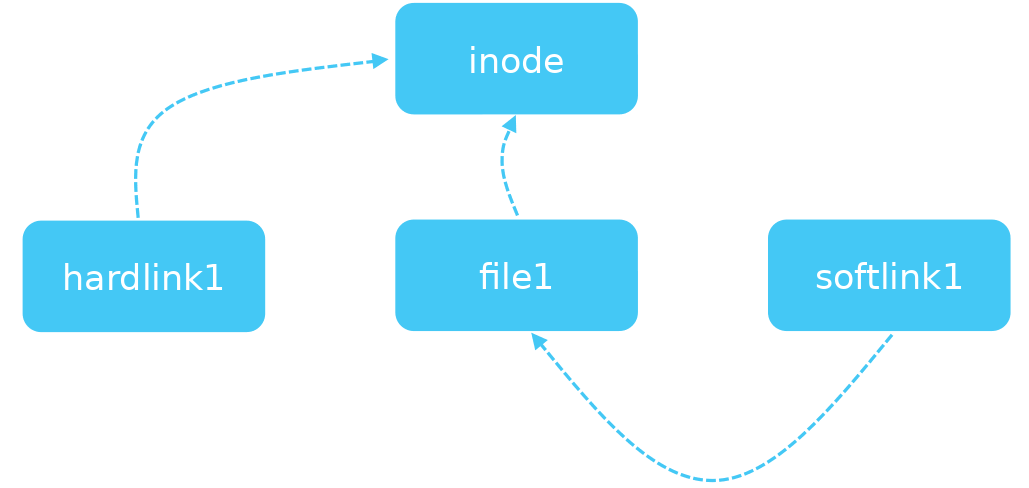
\includegraphics[width=0.5\textwidth]{soft-vs-hard-links.png}
    \caption{Symlink vs Hardlink}
\end{figure}


\subsection{File permissions}

\begin{figure}[H]
    \centering
    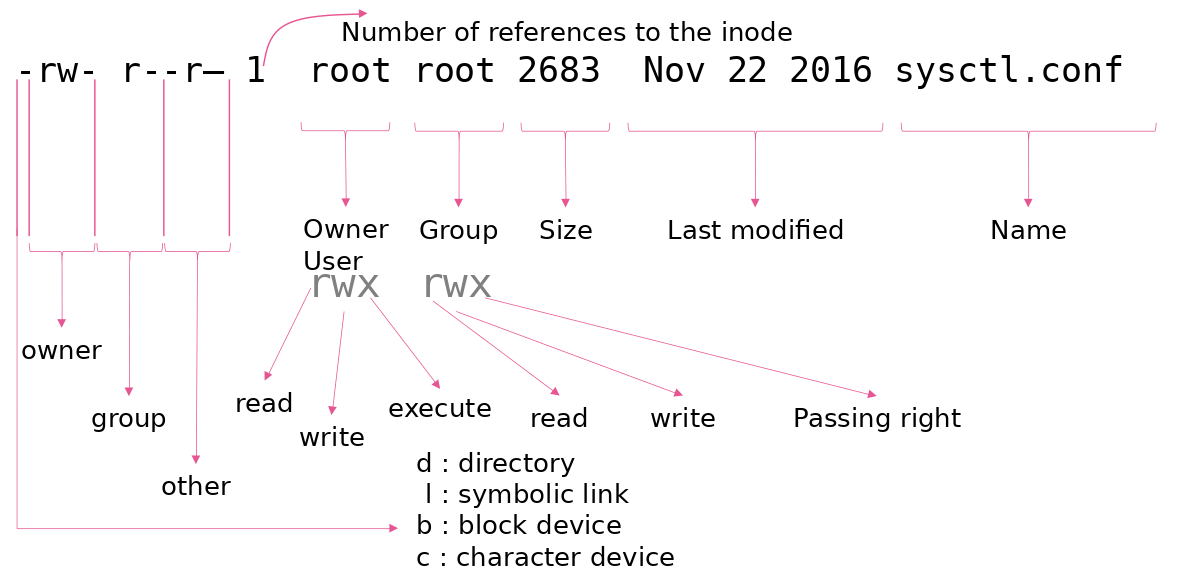
\includegraphics[width=0.8\textwidth]{file-permissions.png}
    \caption{The output of `ls -l' creates this type of output}
\end{figure}

\begin{enumerate}
    \item first character: type of file (directory, symbolic link, block device, character device)
    \item next 9 characters: owner rights, group rights, other rights
    \item next number: number of references to the inode
    \item owner user
    \item owner group
    \item size of file
    \item last modified
    \item name of file
\end{enumerate}

\begin{minted}{bash}
    # change the owner and group of a file or directory
    ~# chown <user>:<group> <file>
    ~# chown root:staff file.txt
    
    # change the rights for a file
    # chmod: change mode
\end{minted}

\begin{figure}[H]
    \centering
    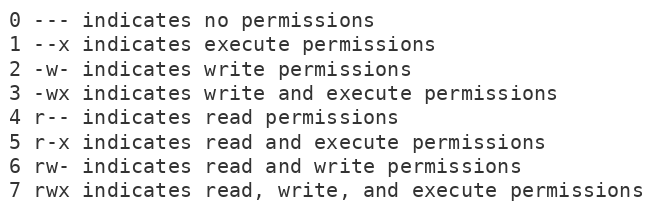
\includegraphics[width=0.5\textwidth]{octal-notation.png}
    \caption{Octal notation}
\end{figure}


\subsection{Overview of basic commands}

Usage and details for these commands: see labs

\begin{itemize}
    \item cat: print contents of file to terminal
    \item cut: cut (structured) input on a specific place: show a certain column, etc\dots
    \item grep: display lines for which the pattern matches
    \item egrep: extended grep, better handling of regular expressions
    \item find: search for files in a hierarchy of files and directories
    \item head: show first lines of file
    \item tail: show last lines of file
    \item less: show the contents of a text file, interactively
    \item man: show manual page for specific command
    \item wc: word count (but also character count, byte counts, newline counts, \dots) for a file
    \item date: show or configure system date and time
    \item cal: show a textual calendar
    \item sort: sort a file
    \item uniq: in a sorted output: count double lines or only show unique lines
\end{itemize}

\subsection{Wooclap}

\begin{itemize}
    \item What is meant by the term journaling for filesystems?
    \item Why is journaling used with filesystems?
    \item Give 2 examples of filesystems under linux that use journaling.
    \item How can you find out which kernel modules are currently loaded?
    \item Which command can you use to load a kernel module? 
    \item And which to 'unload' a kernel module?
    \item How many disks do you need at least to build a RAID10 system? Why?
    \item What is meant by a 'Copy On Write' filesystem?
    \item What are the advantages of a CoW filesystem?
    \item What are snapshots (in the context of storage systems)?
    \item What are the disadvantages of a CoW filesystem?
    \item Why do you still need backup when you have RAID1 and have snapshots?
    \item How can you find out which 'type' is a file? There are no extensions.
    \item What is an inode?
    \item What is the difference between a softlink and a hard link?
    \item At the output of the command ls -la: Which values can the first character of the line have and what do they mean?
    \item At the output of the command ls -la: Which possible values can the 3 groups of 3 characters have to describe the rights?
    \item With what command can you 'change' the 'owner' of a file or directory?
    \item With which command can you 'change' the rights of a file or directory?
    \item What does number 5 mean when you use it to determine file system permissions?
    \item What does number 7 mean when you use that to determine file system rights? Explain why.
    \item Which command do you use to cut structured input at a specific location?
    \item Which command do you use to display the first 16 lines of a text file?
    \item Which command can you use to find out all the modified files from the last 24 hours?
    \item Which command do you use to display the last 12 lines of a text file?
    \item How can you find out how long it has been since a linux system was rebooted?
    \item Which command can you use to get an overview of all daemons that are currently active in your system?
\end{itemize}

\section{Text editors, Piping, Redirection \& Jobs}

\subsection{Text editors}

\begin{itemize}
    \item Emacs (productivity, extensibility)
    \item Nano (simplicity)
    \item Vi / Vim (=VI iMproved) (productivity)
    \item Ne
\end{itemize}

Our choice: Vim

\subsubsection{vi vs vi-improved}

\begin{itemize}
    \item Navigating in vi: HJKL (left, down, up, right)
    \item Navigating in vim: HJKL or arrow keys
\end{itemize}

\begin{figure}[H]
    \centering
    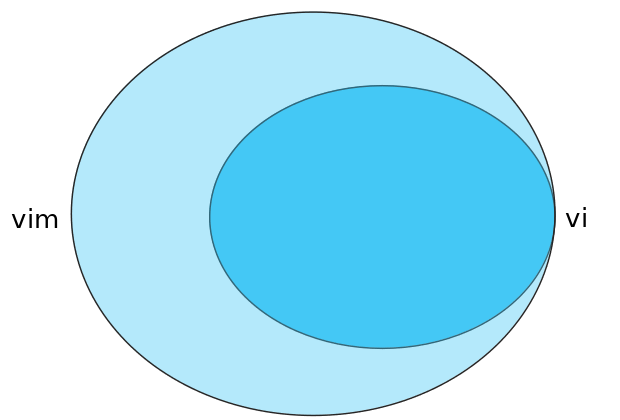
\includegraphics[width=0.5\textwidth]{vi-vim.png}
    \caption{Everything you can do in vi, you can do in vim, and more!}
\end{figure}

\subsubsection{First steps in vim}

\begin{minted}{bash}
# start vim:
$~ vim

# start vim tutorial:
$~ vimtutor
\end{minted}

\begin{itemize}
    \item bottom left of window: the current mode
    \item INSERT = the mode that lets you enter text
    \item Enter INSERT mode: i
    \item Leave INSERT mode and go to normal mode: ESC
    \item Once in normal mode, you can enter commands using `:'
    \item ESC : q $\Rightarrow$ quit
    \item ESC : w $\Rightarrow$ quit
    \item ESC : wq $\Rightarrow$ write and quit
\end{itemize}

\begin{minted}{bash}
# copy a line of text
ESC
# put cursor on the line you want to copy
yy # yank yank: copy a line of text
p # put: paste the copied line

# copy 2 lines of text and paste it 8 times:
ESC 2yy # 2 yank yank: yank 2 lines
8p      # 8 put: paste the copied lines 8 times
\end{minted}

\subsubsection{Search and replace}

You can easily search and replace in a text file, even with regex:

\begin{minted}{bash}
# search and replace the next instance:
:s/old/new

# all instances: TODO: difference between :s and :%s
:s/old/new/g

# all instances between line x and y:
:x,ys/old/new/g

# all instances in a complete file:
:%s/old/new/g

# all instances in whole file, with confirmation:
:%s/old/new/gc

#undo:
(ESC) u
\end{minted}

\subsubsection{Basic editing tricks}

\begin{minted}{bash}
# starting from line 4, indent the next 7 lines:
(ESC) 7>>

# remove indentation on line 10
(ESC) 10gg
<<

# delete line 3
(ESC) 3gg
dd

# delete the next 4 lines
(ESC) 4dd

# enable and disable syntax highlighting in vim
(ESC) : syntax on
(ESC) : syntax off
\end{minted}

For more tricks: see labs

\subsection{Piping}

= Use the output from one command as input for the next command

\begin{minted}{bash}
# sort the music file alphabetically and count the number of occurences of each unique line
sort music.txt | uniq -c

# count the number of unique lines in music.txt
sort music.txt | uniq | wc -l

# count the number of lines in /etc/locale.gen where nl or NL occurs
grep -i nl /etc/locale.gen | wc -l

# count the number of lines in /var/log/syslog where kernel occurs
cat /var/log/syslog | grep kernel | wc –l

# count the number of lines in /var/log/syslog where kernel does NOT occur
cat /var/log/syslog | grep -v kernel | wc –l

# Show of what days there are logs in /var/log/syslog
# the sixth field is the day field:
cat /var/log/syslog | cut -c 6 | uniq

# show the different sources of log entries in /var/log/syslog
# kernel, client, systemd, ...
cat /var/log/syslog | cut -d' ' -f5 | cut -d'[' -f1 | sort | uniq -c
\end{minted}

\subsection{Redirection}

Do not send the output of a command to stdout, but to another location, like a textfile

\begin{minted}{bash}
# to overwrite a file (or create if it doesn't exist)
ls -la > listing.txt

# to append to a file (or create if it doesn't exist)
ls -la >> listing.txt

# these two commands have the same result
cat > textfile.txt
touch textfile.txt

# redirect the output of 'ls -la' to a file with a custom name:
# example: output_2021-03-03
ls -la > output_$(date  +"%F")
\end{minted}

\subsubsection{stdout and stderr}

= 2 important output streams

\begin{itemize}
    \item Normal situation: stdout and stderr appear on the terminal
    \item Redirection: stdout to a file
    \item stderr still prints to the terminal
    \item Redirect stderr: 2> errorfile.txt
\end{itemize}

\begin{figure}[H]
    \centering
    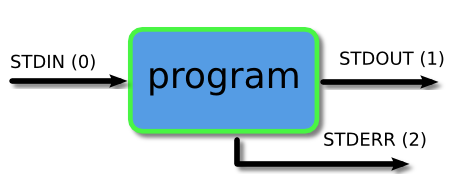
\includegraphics[width=0.5\textwidth]{redirection-std.png}
    \caption{}
\end{figure}

\begin{minted}{bash}
# redirect the output of a command to out.txt 
# and redirect the error of the command to error.txt:
ls -la > out.txt 2> error.txt

# redirect stderr to stdout (&1), and then redirect stdout to a file out.txt:
ls -la > out.txt 2>&1

# redirect both to a file:
ls -la &> out
\end{minted}

\subsubsection{stdin}

\begin{minted}{bash}
# this command prints the amount of lines in a file
wc -l music.txt

# this command does the same
wc -l < music.txt

# this command does the same, but prints the output of wc to out.txt
wc -l < music.txt > out.txt
\end{minted}

\subsection{Jobs and process Management}

When you execute a command: a process is started

\begin{itemize}
    \item Every process gets a process ID (PID)
    \item The init process has PID 0. It starts other processes.
    \item Every process has a parent
    \begin{itemize}
        \item $\Rightarrow$ tree structure of processes
        \item Get insights into this structure with `pstree' (part of the `psmisc' package)
        \item Process stops: exit code is passed to the parent
    \end{itemize}
\end{itemize}

\begin{minted}{bash}
# report a snapshot of current processes
ps

# display a tree of processes
pstree -p
\end{minted}


\subsubsection{Exit codes}

\begin{minted}{bash}
# when a process stops:
# if bash was parent => exit code is passed to bash
# exit code is available in the $? variable:
# read contents of a variable with echo:
echo $?
0

# 0 = ended successfully without errors

# 1 = not ended successfully, there were errors
\end{minted}

\begin{minted}{bash}
# test = verify if you have rights on a file (with -r = read rights)
~$ test -r music.txt

~$ echo $?
0

~$ test -r doesnotexist

# the file doesn't exist, so it exited with code 1:
~$ echo $?
1
\end{minted}

\subsubsection{Combining commands}

= not the same as piping!

\begin{minted}{bash}
# note the difference between & (run in background) and && (combine command)

# one ampersand: run something in the background
test -r test.txt & echo "MCT rocks"

# two ampersands: combine commands
# if the first command exits 0, the second command will work
~# test -r test.txt && echo "MCT rocks"

~# test -r doesnotexist & echo "MCT rocks"

# the first command will exit with code 1
# so the second command will not execute
~# test -r doesnotexist && echo "MCT rocks"
\end{minted}

\subsubsection{Jobs}

A job is a new process originating from the same parent

\begin{minted}{bash}
# start a command as job
tail -f /var/log/syslog &
# output appears on stdout, but process runs as a job in the background

# bring a job to the foreground
fg <index>

# stop the job, but do not terminate:
CTRL-Z
\end{minted}


\subsubsection{Inter-process Communication}

A signal is an asynchronous notification sent to a process or thread within that process
to notify that there has been an event

Signal sent to process $\Rightarrow$ OS interrupts normal execution of that process to deliver the signal

Sending a signal to a process: with the `kill' command:

\begin{minted}{bash}
# not only to kill a process, also to send other signals
kill -s <signal>
\end{minted}

\textbf{Signals}

\begin{itemize}
    \item SIGHUP - 1 - terminate (hang up)
    \item SIGINT - 2 - terminal interrupt signal
    \item SIGKILL - 9 - kill (cannot be caught or ignored)
    \item SIGTERM - 15 - termination signal
\end{itemize}

\begin{minted}{bash}
# send signal 15 to a process with the entered PID
kill -s 15 <pid>

# send signal 15 to the PID of the tail process
kill -s 15 'pidof tail'

# send signal 9 to a process with the entered PID
kill -s 9 <pid>

# kill the process with name 'tail'
pkill tail
\end{minted}


\subsection{Intermezzo: System Load}

= a number which represents the load on a computer system

\begin{itemize}
    \item Completely idle system: system load 0
    \item Each process which uses a resource or is waiting for a resource: system load + 1
    \item Gives an indication of how heavy a computer system is loaded
    \item System load is a snapshot, doesn't say anything
    \begin{itemize}
        \item System load of 17: is that a problem? No.
        \item More interesting: the evolution of the systemload over time
    \end{itemize} 
\end{itemize}

\begin{minted}{bash}
# show the system load of the last minute, last 5 minutes and last 15 minutes:
uptime

# show who is logged on and what they are doing
w

# display linux processes
top
# or better:
htop
\end{minted}

\subsection{Some useful tips}

\subsubsection{With which unique IP-addresses are there open sockets and how many?}

\begin{minted}{bash}
netstat -anpt | awk '{print $5}' | sort | uniq -c
\end{minted}

\subsubsection{TTY}

= Tele TYpewriter
= a terminal which is connected with stdin

\begin{minted}{bash}
# print the filename of the terminal currently connected to standard input:
~$ tty


\end{minted}


\end{document}